\section{}
Consider the following generic closed-loop system:
\begin{figure}[h]
    \centering
    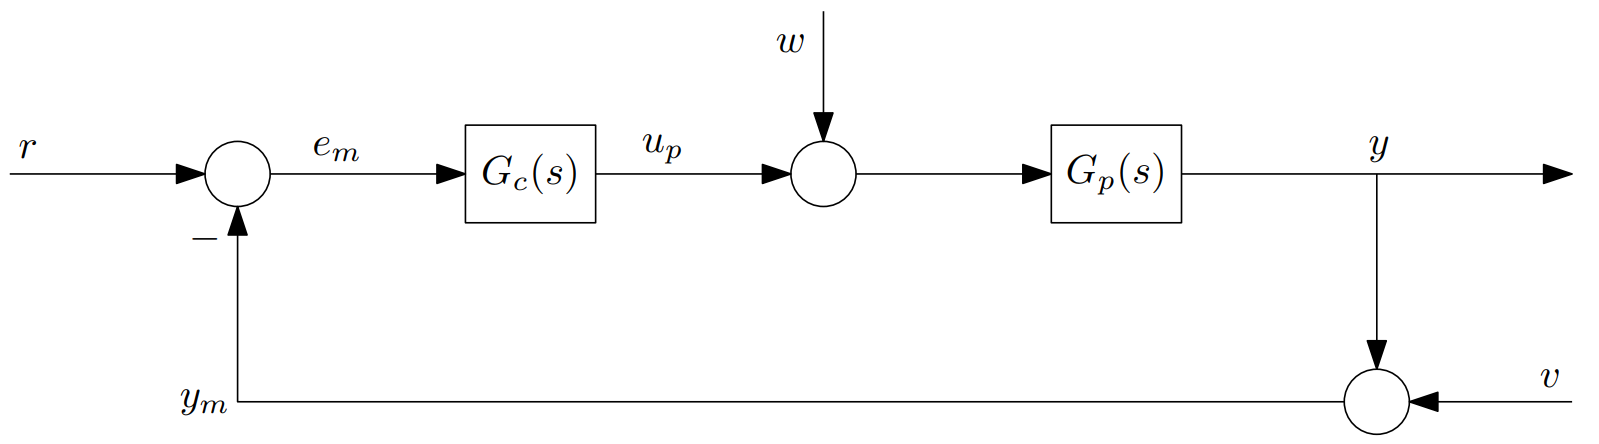
\includegraphics[width=0.8\textwidth]{Questions/Figures/Q4ProblemDiagram.png}
    \caption{Block diagram of the closed-loop system}
    \label{fig:Q4ProblemDiagram}
\end{figure}

% For each of the following cases, verify the stability of the system:
% (a) Gc(s) = 1, Gp(s) = 1
% s + 1
% (b) Gc(s) = 5, Gp(s) = 1
% s
% 2 + 1
% (c) Gc(s) = 1 + 1
% s
% , Gp(s) = s
% (s + 1)(s + 2)
% (d) Gc(s) = s − 1
% s + 1
% , Gp(s) = 1
% s − 2

For each of the following cases, verify the stability of the system:
\begin{enumerate}[label=(\alph*)]
    \item $G_c(s) = 1$, $G_p(s) = \frac{1}{s+1}$
    \item $G_c(s) = 5$, $G_p(s) = \frac{1}{s^2+1}$
    \item $G_c(s) = 1 + \frac{1}{s}$, $G_p(s) = \frac{s}{(s+1)(s+2)}$
    \item $G_c(s) = \frac{s-1}{s+1}$, $G_p(s) = \frac{1}{s-2}$
\end{enumerate}

\subsection{}
By direct computation,
\begin{align*}
    1 + G_c(s)G_p(s) &= 1 + \frac{1}{s+1} = \frac{s+2}{s+1} \\
\end{align*}

The zero is at $s = -2$. Since there are no term cancellations, the system is \textbf{stable.}

\subsection{}
By direct computation,
\begin{align*}
    1 + G_c(s)G_p(s) &= 1 + \frac{5}{s^2+1} = \frac{s^2+6}{s^2+1} \\
\end{align*}

The zeros are at $s = 0 \pm i\sqrt{6}$. Since the real part is 0, the system is \textbf{unstable.}

\subsection{}
By direct computation,
\begin{align*}
    1 + G_c(s)G_p(s) &= 1 + \frac{\cancel{s}\cancel{(s+1)}}{\cancel{s}\cancel{(s+1)}(s+2)}
\end{align*}

Since there are term cancellations in $G_c(s)G_p(s)$, the system is \textbf{unstable.}

\subsection{}
By direct computation,
\begin{align*}
    1 + G_c(s)G_p(s) &= 1 + \frac{s-1}{(s+1)(s-2)} = \frac{s^2-3}{(s+1)(s-2)} \\
\end{align*}
\begin{verbatim}
>> syms s

>> simplifyFraction(1 + (s-1)/((s+1)*(s-2)))
 
ans =
 
(s^2 - 3)/((s + 1)*(s - 2))
\end{verbatim}

The zeros are at $s = \pm \sqrt{3}$. Since the real part is positive, the system is \textbf{unstable.}